\begin{enumerate}[label=\thesubsection.\arabic*, ref=\thesubsection.\theenumi]

\vspace{0.5cm}
% Question 1 (Q8)
\item A fair six-faced dice, with the faces labelled '1', '2', '3', '4', '5', and '6', is rolled thrice. What is the probability of rolling '6' exactly once?
\hfill (CS1~2025)
\begin{enumerate}
	\begin{multicols}{4}
    \item $\dfrac{75}{216}$
    \item $\dfrac{1}{6}$
    \item $\dfrac{1}{18}$
    \item $\dfrac{25}{216}$
	\end{multicols}
\end{enumerate}

\vspace{0.5cm}
\solution
Step 1: Finding the probability mass function (PMF) of a single dice roll \\
The sample space is $S = \{1, 2, 3, 4, 5, 6\}$. Let us define a variable $Y_1$ as follows:
\begin{align}
Y_1 = \begin{cases} 1, & X_1 = 6 \\ 0, & X_1 \neq 6 \end{cases}
\end{align}
Now, the PMF is defined as:
\begin{align}
P_{Y_1}(k) = \begin{cases} \frac{1}{6}, & k = 1 \\ \frac{5}{6}, & k = 0 \end{cases}
\end{align}
Let $p, q$ be $\frac{1}{6}$ and $\frac{5}{6}$ respectively.

Step 2: Applying Z-Transform to find the required PMF for $Y$ \\
Let us define $Y_2$ and $Y_3$ as the random variables for the $2^{\text{nd}}$ and $3^{\text{rd}}$ dice roll, respectively. Let $Y$ denote the random variable for the combined triple dice roll, $Y = Y_1 + Y_2 + Y_3$. \\
From (\ref{eq:CS12025-pmf_ztransform}), writing the Z-Transform for $Y_1$:
\begin{align}
M_{Y_1}(Z) &= E[Z^{-Y_1}] \\
           &= \sum P_{Y_1}(k) Z^{-k} \\
           &= P_{Y_1}(1)Z^{-1} + P_{Y_1}(0)Z^0 \\
           &= p Z^{-1} + q
\end{align}
Since $Y_1, Y_2, Y_3$ are independent events, using (\ref{eq:CS12025-ztransform_sum}), we can write $M_Y(Z) = M_{Y_1}(Z) \, M_{Y_2}(Z) \, M_{Y_3}(Z)$. \\
Therefore,
\begin{align}
M_Y(Z) &= (p Z^{-1} + q)^3 \\
       &= \sum_{k=0}^3 \binom{3}{k} q^{3-k} (p Z^{-1})^k \\
       &= \sum P_Y(k) Z^{-k}
\end{align}
Comparing coefficients, the PMF of $Y$ is:
\begin{align}
P_Y(k) = \binom{3}{k} q^{3-k} p^k
\end{align}

Step 3: Calculating required probability \\
We need the situation where $p$ appears exactly once ($k = 1$). The required term is:
\begin{align}
P_Y(1) &= \binom{3}{1} p^1 q^2 \\
       &= 3 \cdot \left(\frac{1}{6}\right) \left(\frac{5}{6}\right)^2 \\
       &= \frac{75}{216}
\end{align}
Therefore, the required answer is $\frac{75}{216}$.

\vspace{0.5cm}
% Question 2 (Q10)
\item A shop has 4 distinct flavors of ice-cream. One can purchase any number of scoops of any flavor. The order in which the scoops are purchased is inconsequential. If one wants to purchase 3 scoops of ice-cream, in how many ways can one make that purchase?
\hfill (CS1~2025)
\begin{enumerate}
	\begin{multicols}{4}
    \item $4$
    \item $20$
    \item $24$
    \item $48$
	\end{multicols}
\end{enumerate}

\vspace{0.2cm}
\solution
Let $F$ be the event that the chosen coin is the fake coin, and $R$ be the event that it is a regular coin. The prior probabilities of selecting each coin are:
\begin{align}
P(F) &= \frac{1}{5} \\
P(R) &= \frac{4}{5}
\end{align}

Let $H_2$ be the event of getting two heads when the chosen coin is tossed twice. 
The probability of getting two heads with a regular coin is:
\begin{align}
P(H_2 \mid R) = \left(\frac{1}{2}\right) \times \left(\frac{1}{2}\right) = \frac{1}{4}
\end{align}

The probability of getting two heads with the fake coin is:
\begin{align}
P(H_2 \mid F) = 1 \times 1 = 1
\end{align}

Using Bayes' theorem:
\begin{align}
P(F \mid H_2) &= \frac{P(F) P(H_2 \mid F)}{P(F) P(H_2 \mid F) + P(R) P(H_2 \mid R)} \\
              &= \frac{\frac{1}{5} \times 1}{\left(\frac{1}{5} \times 1\right) + \left(\frac{4}{5} \times \frac{1}{4}\right)} \\
              &= 0.50
\end{align}

Therefore, the probability that the coin chosen is the fake coin is $0.50$.

\vspace{0.5cm}
% Question 3 (Q17)
\item $g(\cdot)$ is a function from $A$ to $B$, $f(\cdot)$ is a function from $B$ to $C$, and their composition defined as $f(g(\cdot))$ is a mapping from $A$ to $C$. If $f(\cdot)$ and $f(g(\cdot))$ are onto (surjective) functions, which ONE of the following is TRUE about the function $g(\cdot)$?
\hfill (CS1~2025)
\begin{enumerate}
    \item $g(\cdot)$ must be an onto (surjective) function.
    \item $g(\cdot)$ must be a one-to-one (injective) function.
    \item $g(\cdot)$ must be a bijective function, that is, both one-to-one and onto.
    \item $g(\cdot)$ is not required to be a one-to-one or onto function.
\end{enumerate}

\vspace{0.2cm}
\solution
From (\ref{eq:CS12025-function_composition}), if $f \circ g : A \to C$ is onto, every element in $C$ has a pre-image in $A$. This guarantees that $f$ must be onto, but $g$ does not need to cover all of $B$ if $f$ maps multiple elements of $B$ to the same element in $C$. Thus, $g(\cdot)$ is not required to be one-to-one or onto.

\vspace{0.5cm}
% Question 4 (Q18)
\item Let $G$ be any undirected graph with positive edge weights, and $T$ be a minimum spanning tree of $G$. For any two vertices, $u$ and $v$, let $d_1(u,v)$ and $d_2(u,v)$ be the shortest distances between $u$ and $v$ in $G$ and $T$, respectively. Which ONE of the options is CORRECT for all possible $G$, $T$, $u$ and $v$?
\hfill (CS1~2025)
\begin{enumerate}
	\begin{multicols}{2}
    \item $d_1(u,v) = d_2(u,v)$
    \item $d_1(u,v) \le d_2(u,v)$
    \item $d_1(u,v) \ge d_2(u,v)$
    \item $d_1(u,v) \ne d_2(u,v)$
	\end{multicols}
\end{enumerate}

\vspace{0.2cm}
\solution
Let $d_1(u,v)$ and $d_2(u,v)$ be the shortest distances between $u$ and $v$ in $G$ and $T$, respectively. By (\ref{eq:CS12025-shortest_path_mst}), since every path in $T$ is a valid path in $G$, but $G$ may contain additional edges offering shorter routes:
\begin{align}
d_1(u,v) \le d_2(u,v)
\end{align}

Therefore, option (b) is correct.

\vspace{0.5cm}
% Question 5 (Q20)
\item Consider the following recurrence relation: $T(n) = 2T(n-1) + n 2^n$ for $n>0$, $T(0)=1$. Which ONE of the following options is CORRECT?
\hfill (CS1~2025)
\begin{enumerate}
	\begin{multicols}{2}
    \item $T(n) = \Theta(n^2 2^n)$
    \item $T(n) = \Theta(n 2^n)$
    \item $T(n) = \Theta((\log n)^2 2^n)$
    \item $T(n) = \Theta(4^n)$
	\end{multicols}
\end{enumerate}

\vspace{0.2cm}
\solution
Let $x(n) = T(n)u(n)$ be a causal sequence such that $x(n) = 0$ for $n < 0$ and $x(0) = 1$. The given recurrence relation $T(n) - 2T(n-1) = n 2^n$ for $n > 0$ with initial condition $T(0) = 1$ can be expressed using the unit impulse function $\delta(n)$ as:
\begin{align}
x(n) - 2x(n-1) = n 2^n u(n) + \delta(n)
\end{align}

Taking the Z-transform on both sides:
\begin{align}
X(z) - 2z^{-1}X(z) &= \mathcal{Z}\{n 2^n u(n)\} + \mathcal{Z}\{\delta(n)\}
\end{align}
Using the Z-transform property $\mathcal{Z}\{n a^n u(n)\} = \frac{a z^{-1}}{(1 - a z^{-1})^2}$ for $a = 2$, and $\mathcal{Z}\{\delta(n)\} = 1$:
\begin{align}
X(z)(1 - 2z^{-1}) &= \frac{2z^{-1}}{(1 - 2z^{-1})^2} + 1 \\
\implies X(z) &= \frac{1}{1 - 2z^{-1}} + \frac{2z^{-1}}{(1 - 2z^{-1})^3} \\
             &= \frac{1 - 2z^{-1} + 4z^{-2}}{(1 - 2z^{-1})^3}
\end{align}

Applying partial fraction expansion:
\begin{align}
X(z) = \frac{1}{1 - 2z^{-1}} - \frac{1}{(1 - 2z^{-1})^2} + \frac{2}{(1 - 2z^{-1})^3}
\end{align}

Taking the inverse Z-transform using standard transform pairs:
\begin{itemize}
    \item $\mathcal{Z}^{-1}\left\{\frac{1}{1 - 2z^{-1}}\right\} = 2^n u(n)$
    \item $\mathcal{Z}^{-1}\left\{\frac{1}{(1 - 2z^{-1})^2}\right\} = (n+1)2^n u(n)$
    \item $\mathcal{Z}^{-1}\left\{\frac{1}{(1 - 2z^{-1})^3}\right\} = \frac{(n+1)(n+2)}{2} 2^n u(n)$
\end{itemize}

Substituting these back into $x(n)$:
\begin{align}
x(n) &= 2^n u(n) - (n+1)2^n u(n) + \frac{(n+1)(n+2)}{2} 2^n u(n) \\
     &= 2^n \left[ 1 - (n+1) + \frac{n^2 + 3n + 2}{2} \right] u(n) \\
     &= 2^n \left[ \frac{n^2 + n + 2}{2} \right] u(n) \\
     &= 2^{n-1} (n^2 + n + 2) u(n)
\end{align}

Since $T(n) = x(n)$ for $n \ge 0$:
\begin{align}
T(n) &= 2^{n-1} (n^2 + n + 2) \\
     &= \Theta(n^2 2^n)
\end{align}
Therefore, $T(n) = \Theta(n^2 2^n)$.

The following code gives the following figure (\figref{fig:cs1-2025-q5}).
\begin{lstlisting}[frame=single, basicstyle=\rmfamily, escapeinside={(*@}{@*)}]
(*@\makebox[\dimexpr\linewidth-2\fboxsep-2\fboxrule\relax][c]{codes/compare.py}@*)
\end{lstlisting}
\begin{figure}[H]
    \centering
    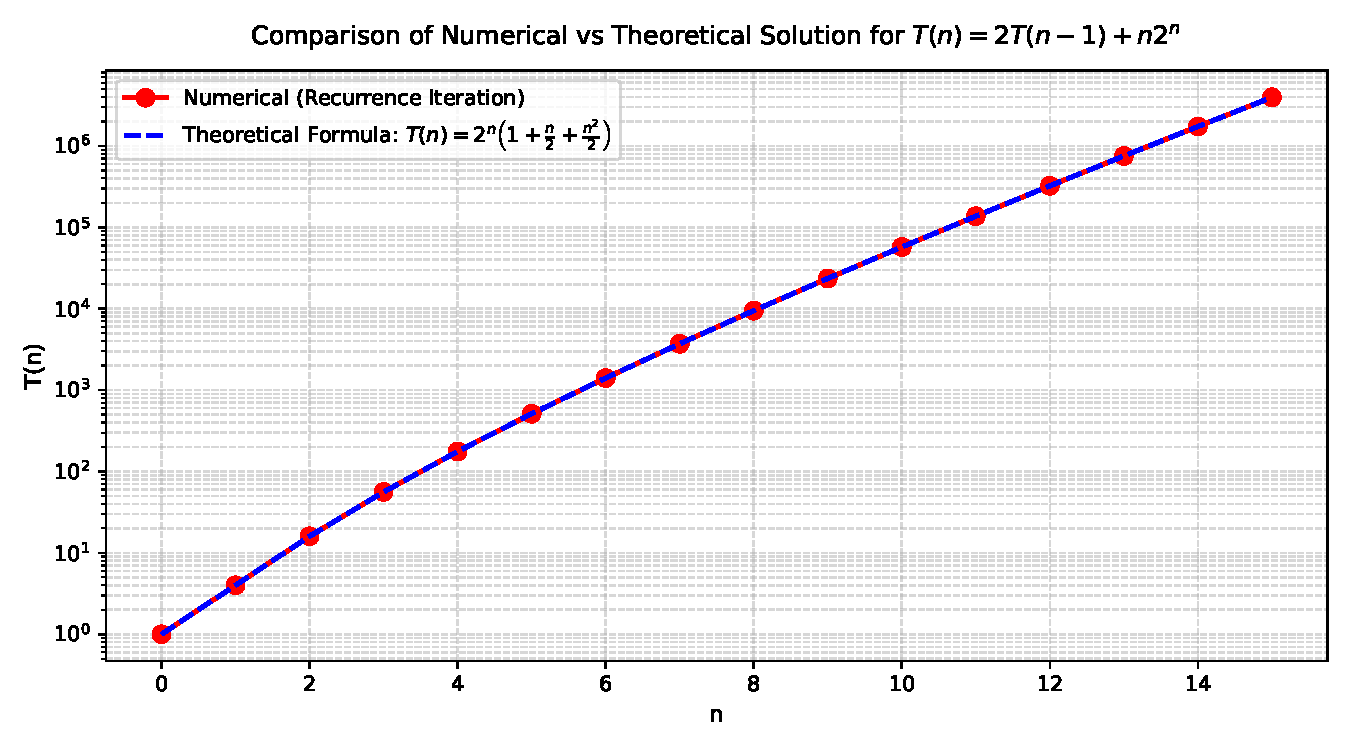
\includegraphics[width=0.75\linewidth]{figs/graph.pdf}
    \caption{Recurrence relation growth analysis}
    \label{fig:cs1-2025-q5}
\end{figure}

\vspace{0.5cm}
% Question 6 (Q23)
\item Consider the given system of linear equations for variables $x$ and $y$, where $k$ is a real-valued constant:
\begin{align*}
x + ky &= 1 \\
kx + y &= -1
\end{align*}
Which of the following option(s) is/are CORRECT?
\hfill (CS1~2025)
\begin{enumerate}
    \item There is exactly one value of $k$ for which the above system of equations has no solution.
    \item There exist an infinite number of values of $k$ for which the system of equations has no solution.
    \item There exists exactly one value of $k$ for which the system of equations has exactly one solution.
    \item There exists exactly one value of $k$ for which the system of equations has an infinite number of solutions.
\end{enumerate}

\vspace{0.2cm}
\solution
The given system of linear equations can be written in matrix form $\mathbf{A}\vec{x} = \vec{b}$ as:
\begin{align}
\begin{bmatrix} 
1 & k \\ 
k & 1 
\end{bmatrix} 
\begin{bmatrix} 
x \\ 
y 
\end{bmatrix} 
= 
\begin{bmatrix} 
1 \\ 
-1 
\end{bmatrix}
\end{align}

Forming the augmented matrix $[\mathbf{A} \mid \vec{b}]$:
\begin{align}
[\mathbf{A} \mid \vec{b}] = 
\begin{bmatrix} 
1 & k & \mid & 1 \\ 
k & 1 & \mid & -1 
\end{bmatrix}
\end{align}

Applying elementary row operation $R_2 \to R_2 - k R_1$ to reduce the matrix to row echelon form:
\begin{align}
[\mathbf{A} \mid \vec{b}] \xrightarrow{R_2 \to R_2 - k R_1} 
\begin{bmatrix} 
1 & k & \mid & 1 \\ 
0 & 1 - k^2 & \mid & -1 - k 
\end{bmatrix}
\end{align}

Let $n = 2$ be the number of variables. From (\ref{eq:CS12025-linear_system_rank}), we analyze the rank of the coefficient matrix $\text{rank}(\mathbf{A})$ and the augmented matrix $\text{rank}([\mathbf{A} \mid \vec{b}])$:

1. Condition for Unique Solution: \\
For a unique solution, $\text{rank}(\mathbf{A}) = \text{rank}([\mathbf{A} \mid \vec{b}]) = n = 2$. \\
This requires the pivot position in the second row to be non-zero:
\begin{align}
1 - k^2 \neq 0 &\implies k^2 \neq 1 \\
               &\implies k \neq 1 \quad \text{and} \quad k \neq -1
\end{align}
Thus, a unique solution exists for infinitely many values of $k$ ($k \in \mathbb{R} \setminus \{1, -1\}$).

2. Condition for Infinite Solutions: \\
For infinitely many solutions, $\text{rank}(\mathbf{A}) = \text{rank}([\mathbf{A} \mid \vec{b}]) < n = 2$, which means $\text{rank}(\mathbf{A}) = \text{rank}([\mathbf{A} \mid \vec{b}]) = 1$. \\
This requires both entries in the second row to vanish simultaneously:
\begin{align}
1 - k^2 = 0 \quad \text{and} \quad -1 - k = 0
\end{align}
From $-1 - k = 0 \implies k = -1$. Substituting $k = -1$ into $1 - k^2$ gives $1 - (-1)^2 = 0$. \\
At $k = -1$, the row echelon form becomes:
\begin{align}
\begin{bmatrix} 
1 & -1 & \mid & 1 \\ 
0 & 0 & \mid & 0 
\end{bmatrix}
\end{align}
Here, $\text{rank}(\mathbf{A}) = 1$ and $\text{rank}([\mathbf{A} \mid \vec{b}]) = 1$. Since $\text{rank}(\mathbf{A}) = \text{rank}([\mathbf{A} \mid \vec{b}]) < 2$, there exists exactly one value of $k$ ($k = -1$) for which the system has an infinite number of solutions.

3. Condition for No Solution (Inconsistent System): \\
For no solution, the system must be inconsistent, which occurs when $\text{rank}(\mathbf{A}) \neq \text{rank}([\mathbf{A} \mid \vec{b}])$ (specifically $\text{rank}(\mathbf{A}) = 1$ and $\text{rank}([\mathbf{A} \mid \vec{b}]) = 2$). \\
This requires $1 - k^2 = 0$ while $-1 - k \neq 0$:
\begin{align}
1 - k^2 = 0 &\implies k = \pm 1 \\
-1 - k \neq 0 &\implies k \neq -1
\end{align}
This gives $k = 1$. At $k = 1$, the row echelon form becomes:
\begin{align}
\begin{bmatrix} 
1 & 1 & \mid & 1 \\ 
0 & 0 & \mid & -2 
\end{bmatrix}
\end{align}
Here, $\text{rank}(\mathbf{A}) = 1$ while $\text{rank}([\mathbf{A} \mid \vec{b}]) = 2$. Since $\text{rank}(\mathbf{A}) \neq \text{rank}([\mathbf{A} \mid \vec{b}])$, there exists exactly one value of $k$ ($k = 1$) for which the system has no solution.

Therefore, options (a) and (d) are correct.

The following code gives the following figure (\figref{fig:cs1-2025-q6}).
\begin{lstlisting}[frame=single, basicstyle=\rmfamily, escapeinside={(*@}{@*)}]
(*@\makebox[\dimexpr\linewidth-2\fboxsep-2\fboxrule\relax][c]{codes/solution.py}@*)
\end{lstlisting}
\begin{figure}[H]
    \centering
    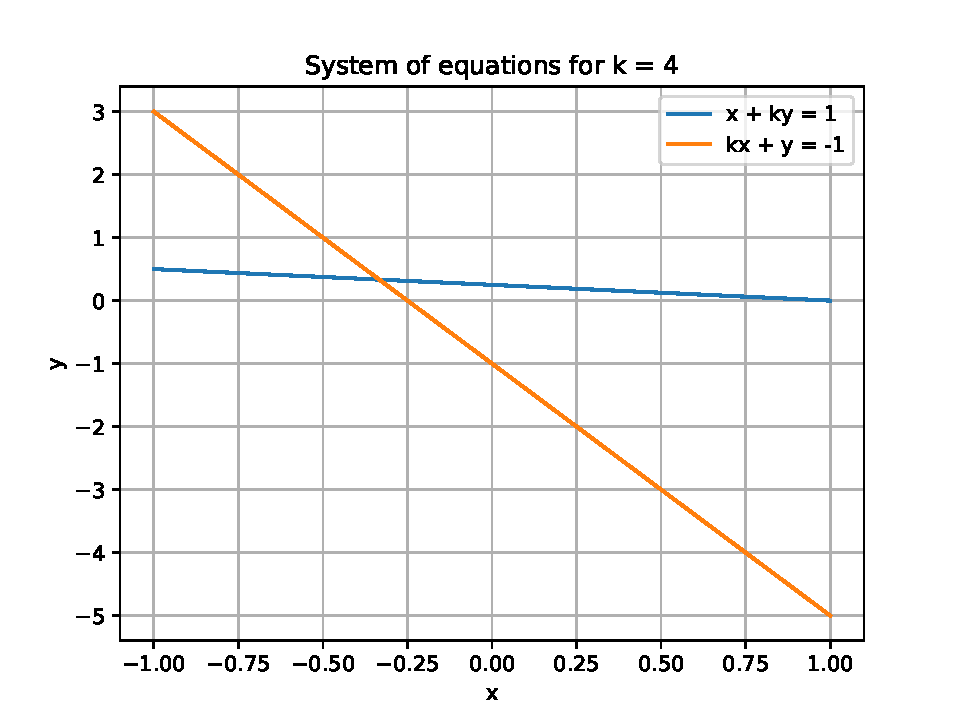
\includegraphics[width=0.75\linewidth]{figs/intersec.pdf}
    \caption{System of linear equations intersection analysis}
    \label{fig:cs1-2025-q6}
\end{figure}

\vspace{0.5cm}
% Question 7 (Q24)
\item Let $X$ be a 3-variable Boolean function that produces output as '1' when at least two of the input variables are '1'. Which of the following statement(s) is/are CORRECT, where $a, b, c, d, e$ are Boolean variables?
\hfill (CS1~2025)
\begin{enumerate}
    \item $X(a,b,X(c,d,e)) = X(X(a,b,c),d,e)$
    \item $X(a,b,X(a,b,c)) = X(a,b,c)$
    \item $X(a,b,X(a,c,d)) = (X(a,b,a) \text{ AND } X(c,d,c))$
    \item $X(a,b,c) = X(a, X(a,b,c), X(a,c,c))$
\end{enumerate}

\vspace{0.2cm}
\solution
The function $X(a,b,c)$ produces output '1' whenever at least two of its three inputs $a, b, c$ are '1'. The truth table describes this relationship:

\begin{center}
\begin{tabular}{|c|c|c|c|}
\hline
$a$ & $b$ & $c$ & $X(a,b,c)$ \\ \hline
0 & 0 & 0 & 0 \\
0 & 0 & 1 & 0 \\
0 & 1 & 0 & 0 \\
0 & 1 & 1 & 1 \\
1 & 0 & 0 & 0 \\
1 & 0 & 1 & 1 \\
1 & 1 & 0 & 1 \\
1 & 1 & 1 & 1 \\ \hline
\end{tabular}

\end{center}

The truth table is generated by the code below:
\begin{lstlisting}[frame=single, basicstyle=\rmfamily, escapeinside={(*@}{@*)}]
(*@\makebox[\dimexpr\linewidth-2\fboxsep-2\fboxrule\relax][c]{codes/truth\_tab.c}@*)
\end{lstlisting}

Mapping the minterms $m(3, 5, 6, 7)$ onto a 3-variable Karnaugh map (Fig.~\ref{fig:q7_kmap}):

\begin{figure}[H]
    \centering
    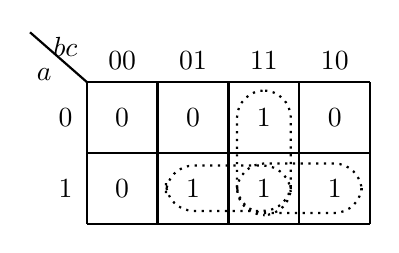
\begin{tikzpicture}[scale=0.9, >=stealth]
    % Grid
    \draw[thick] (0,0) grid (4,2);
    
    % Header diagonal line and labels
    \draw[thick] (0,2) -- (-0.8, 2.7);
    \node at (-0.3, 2.5) {$bc$};
    \node at (-0.6, 2.1) {$a$};
    
    % Column labels
    \node at (0.5, 2.3) {00};
    \node at (1.5, 2.3) {01};
    \node at (2.5, 2.3) {11};
    \node at (3.5, 2.3) {10};
    
    % Row labels
    \node at (-0.3, 1.5) {0};
    \node at (-0.3, 0.5) {1};
    
    % Row 0 values
    \node at (0.5, 1.5) {0};
    \node at (1.5, 1.5) {0};
    \node at (2.5, 1.5) {1};
    \node at (3.5, 1.5) {0};
    
    % Row 1 values
    \node at (0.5, 0.5) {0};
    \node at (1.5, 0.5) {1};
    \node at (2.5, 0.5) {1};
    \node at (3.5, 0.5) {1};
    
    % Group 1: Vertical pair for bc (m3, m7) - Dotted
    \draw[thick, dotted, rounded corners=10pt] (2.12, 0.12) rectangle (2.88, 1.88);
    
    % Group 2: Horizontal pair for ac (m5, m7) - Dotted
    \draw[thick, dotted, rounded corners=10pt] (1.12, 0.18) rectangle (2.88, 0.82);
    
    % Group 3: Horizontal pair for ab (m7, m6) - Dotted
    \draw[thick, dotted, rounded corners=10pt] (2.12, 0.15) rectangle (3.88, 0.85);
\end{tikzpicture}

    \caption{K-map for 3-Variable Majority Function $X(a,b,c)$}
    \label{fig:q7_kmap}
\end{figure}

Grouping adjacent '1's into pairs of size 2:
\begin{itemize}
    \item Group 1 (cells $m_3, m_7$): $bc$
    \item Group 2 (cells $m_5, m_7$): $ac$
    \item Group 3 (cells $m_6, m_7$): $ab$
\end{itemize}
Summing these prime implicants gives the minimized majority Boolean function:
\begin{align}
X(a,b,c) = ab + bc + ca
\end{align}

Evaluating each statement:

\begin{itemize}
    \item Statement (a): $X(a,b,X(c,d,e)) = X(X(a,b,c),d,e)$ \\
    Consider counterexample $a=0, b=0, c=1, d=1, e=1$:
    \begin{align}
    \text{LHS} &= X(0, 0, X(1,1,1)) \\
               &= X(0, 0, 1) \\
               &= 0 \\
    \text{RHS} &= X(X(0,0,1), 1, 1) \\
               &= X(0, 1, 1) \\
               &= 1
    \end{align}
    Since $\text{LHS} \neq \text{RHS}$, statement (a) is incorrect.

    \item Statement (b): $X(a,b,X(a,b,c)) = X(a,b,c)$ \\
    Substituting $X(a,b,c) = ab + bc + ca$:
    \begin{align}
    X(a,b,X(a,b,c)) &= a \cdot b + b \cdot (ab + bc + ca) + a \cdot (ab + bc + ca) \\
                    &= ab + (ab + bc + abc) + (ab + abc + ca) \\
                    &= ab + bc + ca \\
                    &= X(a,b,c)
    \end{align}
    Hence, statement (b) is correct.

    \item Statement (c): $X(a,b,X(a,c,d)) = (X(a,b,a) \text{ AND } X(c,d,c))$ \\
    Evaluating each side:
    \begin{align}
    \text{RHS} &= X(a,b,a) \cdot X(c,d,c) \\
               &= (a + ab) \cdot (c + cd) \\
               &= a \cdot c \\
               &= ac \\
    \text{LHS} &= X(a, b, ac + ad + cd) \\
               &= ab + b(ac + ad + cd) + a(ac + ad + cd) \\
               &= ab + ac + ad + bcd
    \end{align}
    Since $ab + ac + ad + bcd \neq ac$ for general inputs, statement (c) is incorrect.

    \item Statement (d): $X(a,b,c) = X(a, X(a,b,c), X(a,c,c))$ \\
    Note that $X(a,c,c) = ac + cc + ca = c$. Substituting into the RHS:
    \begin{align}
    \text{RHS} &= X(a, X(a,b,c), c) \\
               &= a \cdot X(a,b,c) + c \cdot X(a,b,c) + ca \\
               &= (a + c)(ab + bc + ca) + ca \\
               &= (a^2 b + abc + a^2 c) + (abc + bc^2 + c^2 a) + ca \\
               &= (ab + abc + ac) + (abc + bc + ac) + ac \\
               &= ab + bc + ca \\
               &= X(a,b,c)
    \end{align}
    Hence, statement (d) is correct.
\end{itemize}

Therefore, options (b) and (d) are correct.

\vspace{0.5cm}
% Question 8 (Q25)
\item The number -6 can be represented as 1010 in 4-bit 2's complement representation. Which of the following is/are CORRECT 2's complement representation(s) of -6?
\hfill (CS1~2025)
\begin{enumerate}
	\begin{multicols}{2}
    \item 1000 1010 in 8-bits
    \item 1111 1010 in 8-bits
    \item 1000 0000 0000 1010 in 16-bits
    \item 1111 1111 1111 1010 in 16-bits
	\end{multicols}
\end{enumerate}

\vspace{0.2cm}
\solution
For the 8-bit representation, $+6$ is expressed as $0000\,0110_2$. Flipping all the bits gives the 1's complement $1111\,1001_2$. Adding $1$ yields the 2's complement:
\begin{align}
1111\,1001_2 + 1 = 1111\,1010_2
\end{align}

For the 16-bit representation, $+6$ is expressed as $0000\,0000\,0000\,0110_2$. Flipping all the bits gives the 1's complement $1111\,1111\,1111\,1001_2$. Adding $1$ yields the 2's complement:
\begin{align}
1111\,1111\,1111\,1001_2 + 1 = 1111\,1111\,1111\,1010_2
\end{align}

Therefore, options (b) and (d) are correct.

\vspace{0.5cm}
% Question 9 (Q30)
\item Let $S$ be the set of all ternary strings defined over the alphabet $\{a, b, c\}$. Consider all strings in $S$ that contain at least one occurrence of two consecutive symbols, that is, "aa", "bb" or "cc". The number of such strings of length 5 that are possible is \underline{\hspace{1cm}}.
\hfill (CS1~2025)

\vspace{0.2cm}
\solution
The total number of ternary strings of length 5 is:
\begin{align}
N_{\text{total}} = 3^5 = 243
\end{align}
Using (\ref{eq:CS12025-no_consec_strings}), the number of ternary strings of length 5 with NO consecutive identical symbols is:
\begin{align}
N_{\text{no\_consec}} &= 3 \times (3-1)^{5-1} \\
                      &= 3 \times 2^4 \\
                      &= 48
\end{align}
Subtracting from the total gives the required count:
\begin{align}
N_{\text{consecutive}} &= 243 - 48 \\
                       &= 195
\end{align}

\vspace{0.5cm}
% Question 10 (Q31)
\item Consider the given function $f(x)$:
\begin{align*}
f(x) = \begin{cases} ax + b, & \text{for } x < 1 \\ x^3 + x^2 + 1, & \text{for } x \ge 1 \end{cases}
\end{align*}
If the function is differentiable everywhere, the value of $b$ must be \underline{\hspace{1cm}}.
\hfill (CS1~2025)

\vspace{0.2cm}
\solution
For a function $f(x)$ to be differentiable everywhere, it must be both continuous and differentiable at the boundary point $x = 1$.

For continuity at $x = 1$, the left-hand limit, right-hand limit, and function value $f(1)$ must be equal:
\begin{align}
\lim_{x \to 1^-} f(x) &= \lim_{x \to 1^-} (ax + b) = a + b \label{eq:cont_lhs} \\
\lim_{x \to 1^+} f(x) &= \lim_{x \to 1^+} (x^3 + x^2 + 1) = 3 \\
f(1) &= 1^3 + 1^2 + 1 = 3
\end{align}
Equating the left-hand and right-hand limits gives:
\begin{align}
a + b = 3 \label{eq:cont}
\end{align}

Differentiating $f(x)$ piecewise for $x \neq 1$:
\begin{align}
f'(x) = \begin{cases} a, & x < 1 \\ 3x^2 + 2x, & x > 1 \end{cases}
\end{align}

By (\ref{eq:CS12025-piecewise_differentiability}), for $f(x)$ to be differentiable at $x = 1$, the left-hand derivative and right-hand derivative must be equal:
\begin{align}
\lim_{x \to 1^-} f'(x) &= a \\
\lim_{x \to 1^+} f'(x) &= \lim_{x \to 1^+} (3x^2 + 2x) \\
                       &= 3(1)^2 + 2(1) \\
                       &= 5
\end{align}
Equating the left-hand and right-hand derivatives gives:
\begin{align}
a = 5
\end{align}

Substituting $a = 5$ into \eqref{eq:cont}:
\begin{align}
5 + b = 3 &\implies b = 3 - 5 \\
          &\implies b = -2
\end{align}

Therefore, the required value of $b$ is $-2$.

The following code gives the following figure (\figref{fig:cs1-2025-q10}).
\begin{lstlisting}[frame=single, basicstyle=\rmfamily, escapeinside={(*@}{@*)}]
(*@\makebox[\dimexpr\linewidth-2\fboxsep-2\fboxrule\relax][c]{codes/verify\_31.py}@*)
\end{lstlisting}
\begin{figure}[H]
    \centering
    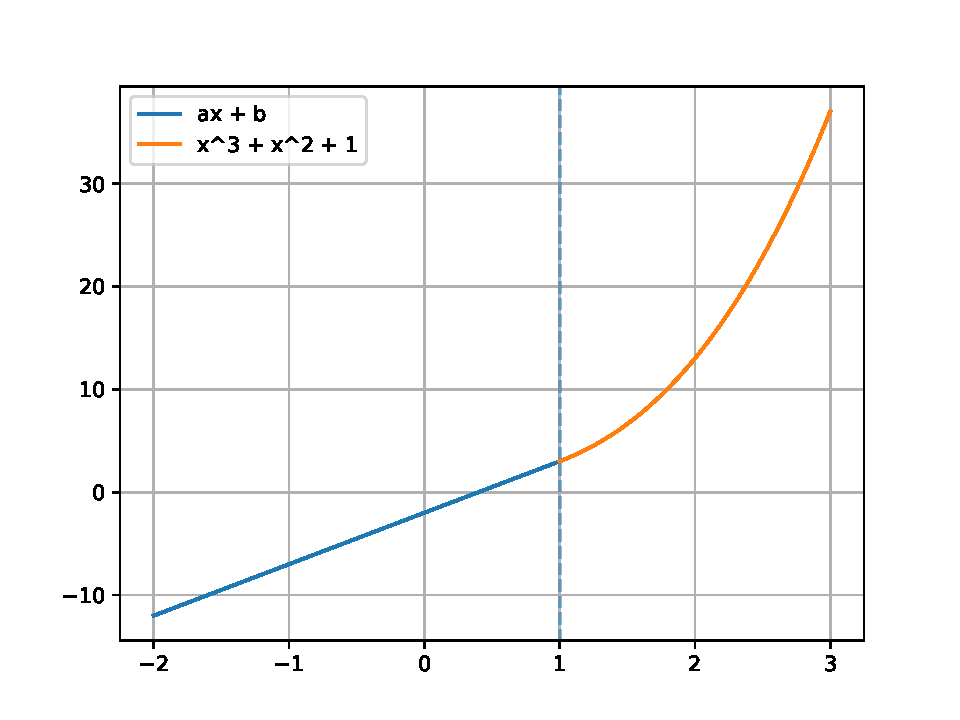
\includegraphics[width=0.75\linewidth]{figs/plot.pdf}
    \caption{Function differentiability plot}
    \label{fig:cs1-2025-q10}
\end{figure}

\vspace{0.5cm}
% Question 11 (Q32)
\item A box contains 5 coins: 4 regular coins and 1 fake coin. When a regular coin is tossed, the probability $P(\text{head})=0.5$ and for a fake coin, $P(\text{head})=1$. You pick a coin at random and toss it twice, and get two heads. The probability that the coin you have chosen is the fake coin is \underline{\hspace{1cm}}.
\hfill (CS1~2025)

\vspace{0.2cm}
\solution
Let $F$ be the event that the chosen coin is the fake coin, and $R$ be the event that it is a regular coin. 
The prior probabilities of selecting each coin are $P(F) = \frac{1}{5}$ and $P(R) = \frac{4}{5}$.
Let $H_2$ be the event of getting two heads when tossing the chosen coin twice.

The probability of getting two heads given a regular coin is:
\begin{align}
P(H_2 \mid R) = (0.5)^2 = 0.25
\end{align}

The probability of getting two heads given a fake coin is:
\begin{align}
P(H_2 \mid F) = (1.0)^2 = 1.0
\end{align}

Using Bayes' theorem:
\begin{align}
P(F \mid H_2) &= \frac{P(F) P(H_2 \mid F)}{P(F) P(H_2 \mid F) + P(R) P(H_2 \mid R)} \\
              &= \frac{\frac{1}{5} \times 1.0}{\left(\frac{1}{5} \times 1.0\right) + \left(\frac{4}{5} \times 0.25\right)} \\
              &= \frac{0.2}{0.2 + 0.2} \\
              &= 0.50
\end{align}

Therefore, the probability that the chosen coin is the fake coin is $0.50$.

\vspace{0.5cm}
% Question 12 (Q33)
\item The pseudocode of a function \texttt{fun()} is given below:
\begin{lstlisting}[language=C]
fun (int A[0,...,n-1]) {
    for i = 0 to n-2
        for j = 0 to n-i-2
            if (A[j] > A[j+1])
                then swap A[j] and A[j+1]
}
\end{lstlisting}
Let $A[0,\dots,29]$ be an array storing 30 distinct integers in descending order. The number of swap operations that will be performed, if the function \texttt{fun()} is called with $A[0,\dots,29]$ as argument, is \underline{\hspace{1cm}}.
\hfill (CS1~2025)

\vspace{0.2cm}
\solution
The given pseudocode implements the standard Bubble Sort algorithm to sort an array in ascending order.

When an array of size $n = 30$ is given in strictly descending order, it represents the worst-case scenario where every adjacent pair comparison $A[j] > A[j+1]$ evaluates to true. Consequently, a swap operation is performed on every comparison.

Using (\ref{eq:CS12025-bubble_sort_swaps}):
\begin{align}
\text{Total Swaps} &= \frac{n(n - 1)}{2} \\
                   &= \frac{30 \times (30 - 1)}{2} \\
                   &= \frac{30 \times 29}{2} \\
                   &= 435
\end{align}

Therefore, the total number of swap operations performed is $435$.

The following code generates a random array A and performs the given function:
\begin{lstlisting}[frame=single, basicstyle=\rmfamily, escapeinside={(*@}{@*)}]
(*@\makebox[\dimexpr\linewidth-2\fboxsep-2\fboxrule\relax][c]{codes/verify\_33.c}@*)
\end{lstlisting}

\vspace{0.5cm}
% Question 13 (Q34)
\item Consider the following C program:
\begin{lstlisting}[language=C]
#include <stdio.h>

void foo (int *p, int x) {
    *p = x;
}

int main() {
    int *z;
    int a = 20, b = 25;
    z = &a;
    foo (z, b);
    printf ("%d", a);
    return 0;
}
\end{lstlisting}
The output of the given C program is \underline{\hspace{1cm}}.
\hfill (CS1~2025)

\vspace{0.2cm}
\solution
In \texttt{main()}, pointer \texttt{z} stores the address of variable \texttt{a}. Passing \texttt{z} to \texttt{foo()} allows \texttt{*p = x} to modify variable \texttt{a} directly to $25$. Thus, \texttt{printf} outputs $25$.

\vspace{0.5cm}
% Question 14 (Q41)
\item Let $A$ be a $2\times2$ matrix as given:
\begin{align*}
A = \begin{bmatrix} 1 & 1 \\ 1 & -1 \end{bmatrix}
\end{align*}
What are the eigenvalues of the matrix $A^{13}$?
\hfill (CS1~2025)
\begin{enumerate}
	\begin{multicols}{2}
    \item $1, -1$
    \item $2\sqrt{2}, -2\sqrt{2}$
    \item $4\sqrt{2}, -4\sqrt{2}$
    \item $64\sqrt{2}, -64\sqrt{2}$
	\end{multicols}
\end{enumerate}

\vspace{0.2cm}
\solution
The characteristic equation of $A$ is $\det(A - \lambda I) = (1-\lambda)(-1-\lambda) - 1 = \lambda^2 - 2 = 0 \implies \lambda = \pm \sqrt{2}$. \\
From (\ref{eq:CS12025-eigenvalue_power}):
\begin{align}
\lambda^{13} &= (\pm \sqrt{2})^{13} \\
             &= \pm (\sqrt{2})^{12} \cdot \sqrt{2} \\
             &= \pm 2^6 \sqrt{2} \\
             &= \pm 64\sqrt{2}
\end{align}

The solution can be verified by the given code:
\begin{lstlisting}[frame=single, basicstyle=\rmfamily, escapeinside={(*@}{@*)}]
(*@\makebox[\dimexpr\linewidth-2\fboxsep-2\fboxrule\relax][c]{codes/eigenval.py}@*)
\end{lstlisting}

\vspace{0.5cm}
% Question 15 (Q42)
\item Consider the following four variable Boolean function in sum-of-product form:
\begin{align*}
F(b_3,b_2,b_1,b_0) = \Sigma(0,2,4,8,10,11,12)
\end{align*}
where the value of the function is computed by considering $b_3 b_2 b_1 b_0$ as a 4-bit binary number, where $b_3$ denotes the most significant bit and $b_0$ denotes the least significant bit. Note that there are no don't care terms. Which ONE of the following options is the CORRECT minimized Boolean expression for $F$?
\hfill (CS1~2025)
\begin{enumerate}
	\begin{multicols}{2}
    \item $\overline{b}_1\overline{b}_0 + \overline{b}_2\overline{b}_0 + b_1\overline{b}_2 b_3$
    \item $\overline{b}_1\overline{b}_0 + \overline{b}_2\overline{b}_0$
    \item $\overline{b}_2\overline{b}_0 + b_1 b_2 b_3$
    \item $\overline{b}_0\overline{b}_2 + \overline{b}_3$
	\end{multicols}
\end{enumerate}

\vspace{0.2cm}
\solution
Truth Table for the 4-variable Boolean function $F(b_3, b_2, b_1, b_0) = \Sigma(0, 2, 4, 8, 10, 11, 12)$:

\begin{center}
\begin{tabular}{|c|c|c|c|c|}
\hline
$b_3$ & $b_2$ & $b_1$ & $b_0$ & $F$ \\ \hline
0 & 0 & 0 & 0 & 1 \\
0 & 0 & 0 & 1 & 0 \\
0 & 0 & 1 & 0 & 1 \\
0 & 0 & 1 & 1 & 0 \\
0 & 1 & 0 & 0 & 1 \\
0 & 1 & 0 & 1 & 0 \\
0 & 1 & 1 & 0 & 0 \\
0 & 1 & 1 & 1 & 0 \\ \hline
\end{tabular}
\quad
\begin{tabular}{|c|c|c|c|c|}
\hline
$b_3$ & $b_2$ & $b_1$ & $b_0$ & $F$ \\ \hline
1 & 0 & 0 & 0 & 1 \\
1 & 0 & 0 & 1 & 0 \\
1 & 0 & 1 & 0 & 1 \\
1 & 0 & 1 & 1 & 1 \\
1 & 1 & 0 & 0 & 1 \\
1 & 1 & 0 & 1 & 0 \\
1 & 1 & 1 & 0 & 0 \\
1 & 1 & 1 & 1 & 0 \\ \hline
\end{tabular}

\end{center}

The following code generates the truth table:
\begin{lstlisting}[frame=single, basicstyle=\rmfamily, escapeinside={(*@}{@*)}]
(*@\makebox[\dimexpr\linewidth-2\fboxsep-2\fboxrule\relax][c]{codes/truth\_tab\_15.c}@*)
\end{lstlisting}

Karnaugh Map (K-map) and Expression Minimization are shown in Fig.~\ref{fig:q15_kmap}:

\begin{figure}[H]
    \centering
    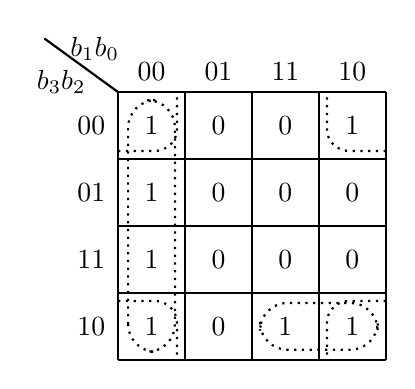
\begin{tikzpicture}[scale=0.85, >=stealth]
    % Grid
    \draw[thick] (0,0) grid (4,4);
    
    % Header diagonal line and labels
    \draw[thick] (0,4) -- (-1.1, 4.8);
    \node at (-0.35, 4.65) {$b_1 b_0$};
    \node at (-0.85, 4.15) {$b_3 b_2$};
    
    % Column labels
    \node at (0.5, 4.3) {00};
    \node at (1.5, 4.3) {01};
    \node at (2.5, 4.3) {11};
    \node at (3.5, 4.3) {10};
    
    % Row labels
    \node at (-0.4, 3.5) {00};
    \node at (-0.4, 2.5) {01};
    \node at (-0.4, 1.5) {11};
    \node at (-0.4, 0.5) {10};
    
    % Row 00 values (m0, m1, m3, m2)
    \node at (0.5, 3.5) {1};
    \node at (1.5, 3.5) {0};
    \node at (2.5, 3.5) {0};
    \node at (3.5, 3.5) {1};
    
    % Row 01 values (m4, m5, m7, m6)
    \node at (0.5, 2.5) {1};
    \node at (1.5, 2.5) {0};
    \node at (2.5, 2.5) {0};
    \node at (3.5, 2.5) {0};
    
    % Row 11 values (m12, m13, m15, m14)
    \node at (0.5, 1.5) {1};
    \node at (1.5, 1.5) {0};
    \node at (2.5, 1.5) {0};
    \node at (3.5, 1.5) {0};
    
    % Row 10 values (m8, m9, m11, m10)
    \node at (0.5, 0.5) {1};
    \node at (1.5, 0.5) {0};
    \node at (2.5, 0.5) {1};
    \node at (3.5, 0.5) {1};
    
    % Group 1: Full Column 00 (m0, m4, m12, m8) - Dotted
    \draw[thick, dotted, rounded corners=10pt] (0.15, 0.12) rectangle (0.85, 3.88);
    
    % Group 2: 4 Corner arcs (m0, m2, m8, m10) - Dotted
    \draw[thick, dotted, rounded corners=8pt] (0.0, 3.12) -- (0.88, 3.12) -- (0.88, 4.0);
    \draw[thick, dotted, rounded corners=8pt] (4.0, 3.12) -- (3.12, 3.12) -- (3.12, 4.0);
    \draw[thick, dotted, rounded corners=8pt] (0.0, 0.88) -- (0.88, 0.88) -- (0.88, 0.0);
    \draw[thick, dotted, rounded corners=8pt] (4.0, 0.88) -- (3.12, 0.88) -- (3.12, 0.0);
    
    % Group 3: Horizontal Pair in Row 10 (m11, m10) - Dotted
    \draw[thick, dotted, rounded corners=10pt] (2.12, 0.15) rectangle (3.88, 0.85);
\end{tikzpicture}

    \caption{K-map for 4-Variable Boolean Function $F(b_3,b_2,b_1,b_0)$}
    \label{fig:q15_kmap}
\end{figure}

Grouping minterms into prime implicants:
\begin{itemize}
    \item Group 1 (Column $b_1 b_0 = 00$, minterms $m_0, m_4, m_{12}, m_8$): $\overline{b}_1 \overline{b}_0$
    \item Group 2 (4 Corners, minterms $m_0, m_2, m_8, m_{10}$): $\overline{b}_2 \overline{b}_0$
    \item Group 3 (Pair, minterms $m_{10}, m_{11}$): $b_3 \overline{b}_2 b_1$
\end{itemize}

Summing these prime implicants gives the minimized Boolean expression:
\begin{align}
F = \overline{b}_1 \overline{b}_0 + \overline{b}_2 \overline{b}_0 + b_3 \overline{b}_2 b_1
\end{align}

Therefore, option (a) is correct.

\vspace{0.5cm}
% Question 16 (Q43)
\item Let $G(V,E)$ be an undirected and unweighted graph with 100 vertices. Let $d(u,v)$ denote the number of edges in a shortest path between vertices $u$ and $v$ in $V$. Let the maximum value of $d(u,v)$, $u,v\in V$ such that $u\ne v$ be 30. Let $T$ be any breadth-first-search tree of $G$. Which ONE of the given options is CORRECT for every such graph $G$?
\hfill (CS1~2025)
\begin{enumerate}
	\begin{multicols}{2}
    \item The height of $T$ is exactly 15.
    \item The height of $T$ is exactly 30.
    \item The height of $T$ is at least 15.
    \item The height of $T$ is at least 30.
	\end{multicols}
\end{enumerate}

\vspace{0.2cm}
\solution
Concept:
The diameter of a graph is the maximum shortest path distance between any pair of vertices. For any breadth-first-search (BFS) tree $T$ rooted at a vertex $r$, the distance from $r$ to any vertex is at most the tree's height $h(T)$. By the triangle inequality, the distance between any two vertices $u$ and $v$ is bounded by $d(u,v) \le d(r,u) + d(r,v) \le 2h(T)$.

Solution:
Given that the maximum shortest path distance in $G$ is 30, from (\ref{eq:CS12025-bfs_tree_height}):
\begin{align}
30 &\le 2h(T) \\
h(T) &\ge 15
\end{align}

Therefore, the height of $T$ is at least 15, making option (c) correct.

\vspace{0.5cm}
% Question 17 (Q49)
\item $A=\{0,1,2,3,\dots\}$ is the set of non-negative integers. Let $F$ be the set of functions from $A$ to itself. For any two functions, $f_1, f_2 \in F$ we define
\begin{align*}
(f_1 \odot f_2)(n) = f_1(n) + f_2(n)
\end{align*}
for every number $n$ in $A$. Which of the following is/are CORRECT about the mathematical structure $(F, \odot)$?
\hfill (CS1~2025)
\begin{enumerate}
	\begin{multicols}{2}
    \item $(F, \odot)$ is an Abelian group.
    \item $(F, \odot)$ is an Abelian monoid.
    \item $(F, \odot)$ is a non-Abelian group.
    \item $(F, \odot)$ is a non-Abelian monoid.
	\end{multicols}
\end{enumerate}

\vspace{0.2cm}
\solution
For the set of functions $F$ mapping $A = \{0, 1, 2, 3, \dots\}$ to itself under the operation $(f_1 \odot f_2)(n) = f_1(n) + f_2(n)$:
\begin{itemize}
    \item Closure and Associativity: The addition of non-negative integers is closed and associative, making $(F, \odot)$ an associative structure.
    \item Commutativity: Since $f_1(n) + f_2(n) = f_2(n) + f_1(n)$, the operation is commutative (Abelian).
    \item Identity Element: The zero function $e(n) = 0$ serves as the identity element since $f(n) + 0 = f(n)$.
    \item Inverses: Non-zero functions do not have inverse elements in $F$ because the codomain consists solely of non-negative integers, meaning negative values required for additive inverses are absent.
\end{itemize}

Since it satisfies monoid axioms and commutativity without having inverses, $(F, \odot)$ is an Abelian monoid. Therefore, option (b) is correct.

\vspace{0.5cm}
% Question 18 (Q52)
\item Refer to the given 3-address code sequence. This code sequence is split into basic blocks. The number of basic blocks is \underline{\hspace{1cm}}.
\hfill (CS1~2025)
\begin{lstlisting}[language=C]
1001: i = 1
1002: j = 1
1003: t1 = 10 * i
1004: t2 = t1 + j
1005: t3 = 8 * t2
1006: t4 = t3 - 88
1007: a[t4] = 0.0
1008: j = j + 1
1009: if j <= 10 goto 1003
1010: i = i + 1
1011: if i <= 10 goto 1002
1012: i = 1
1013: t5 = i - 1
1014: t6 = 88 * t5
1015: a[t6] = 1.0
1016: i = i + 1
1017: if i <= 10 goto 1013
\end{lstlisting}

\vspace{0.2cm}
\solution
To find the number of basic blocks, we first identify the code's leaders using (\ref{eq:CS12025-basic_block_leaders}):
\begin{itemize}
    \item First Instruction: Instruction $1001$ starts the program, so it is automatically a leader.
    \item Jump Targets: Instructions $1002$, $1003$, and $1013$ are leaders because they are the destination targets of conditional jump (\texttt{goto}) statements in the loops.
    \item Instructions Following Jumps: Instructions $1010$ and $1012$ are leaders because they immediately follow jump instructions (lines $1009$ and $1011$), where control flow falls through when a loop condition becomes false.
\end{itemize}

Collecting these leaders gives the set $\{1001, 1002, 1003, 1010, 1012, 1013\}$. 

Since there are $6$ distinct leaders, the given 3-address code sequence is split into $6$ basic blocks.

\vspace{0.5cm}
% Question 19 (Q55)
\item Consider the following database tables of a sports league:
\begin{itemize}
    \item \texttt{player (pid, pname, age)}
    \item \texttt{coach (cid, cname)}
    \item \texttt{team (tid, tname, city, cid)}
    \item \texttt{members (pid, tid)}
\end{itemize}
An instance of the table and an SQL query are given below.

\vspace{0.2cm}
\begin{center}
\begin{tabular}{|c|c|c|}
\hline
pid & pname & age \\ \hline
1 & Jasprit & 31 \\
2 & Atharva & 24 \\
3 & Ishan & 26 \\
4 & Axar & 30 \\ \hline
\end{tabular}

\end{center}

\begin{center}
\begin{tabular}{|c|c|}
\hline
cid & cname \\ \hline
101 & Ricky \\
102 & Mark \\
103 & Trevor \\ \hline
\end{tabular}

\end{center}

\begin{center}
\begin{tabular}{|c|c|c|c|}
\hline
tid & tname & city & cid \\ \hline
10 & MI & Mumbai & 102 \\
20 & DC & Delhi & 101 \\
30 & PK & Mohali & 103 \\ \hline
\end{tabular}

\end{center}

\begin{center}
\begin{tabular}{|c|c|}
\hline
pid & tid \\ \hline
1 & 10 \\
2 & 30 \\
3 & 10 \\
4 & 20 \\ \hline
\end{tabular}

\end{center}

\vspace{0.3cm}
\begin{lstlisting}[language=SQL]
SELECT MIN (P.age)
FROM player P
WHERE P.pid IN (
    SELECT M.pid
    FROM team T, coach C, members M
    WHERE C.cname = 'Mark'
      AND T.cid = C.cid
      AND M.tid = T.tid
)
\end{lstlisting}
The value returned by the given SQL query is \underline{\hspace{1cm}}.
\hfill (CS1~2025)

\vspace{0.2cm}
\solution
Coach 'Mark' has \texttt{cid = 102}, corresponding to team \texttt{tid = 10}. Players in team 10 are \texttt{pid = 1} (age 31) and \texttt{pid = 3} (age 26). The minimum age is $\min(31, 26) = 26$.

\vspace{0.5cm}
% Question 20 (Q56)
\item Suppose a 5-bit message is transmitted from a source to a destination through a noisy channel. The probability that a bit of the message gets flipped during transmission is 0.01. Flipping of each bit is independent of one another. The probability that the message is delivered error-free to the destination is \underline{\hspace{1cm}}.
\hfill (CS1~2025)

\vspace{0.2cm}
\solution
To find the probability that the 5-bit message is delivered error-free using PMFs (referencing (\ref{eq:CS12025-pmf_ztransform})), Z-transforms (referencing (\ref{eq:CS12025-ztransform_sum})), and convolution:

\begin{enumerate}
    \item PMF for a Single Bit:
    Let $X_i$ be the random variable representing the number of errors in the $i$-th bit, where $X_i \in \{0, 1\}$. The probability of a bit being correct is $1 - 0.01 = 0.99$ and being flipped is $0.01$. The PMF is given by $P(X_i = 0) = 0.99$ and $P(X_i = 1) = 0.01$.

    \item Z-Transform for a Single Bit:
    The probability generating function (Z-transform) for a single bit error distribution is:
    \begin{align}
    G_i(z) &= E[z^{X_i}] \\
           &= P(X_i = 0)z^0 + P(X_i = 1)z^1 \\
           &= 0.99 + 0.01z
    \end{align}

    \item Convolution via Z-Transform for 5 Bits:
    For 5 independent bits, the total number of errors is $Y = X_1 + X_2 + X_3 + X_4 + X_5$. Convolution of independent error distributions corresponds to multiplying their individual generating functions:
    \begin{align}
    G_Y(z) &= \prod_{i=1}^{5} G_i(z) \\
    G_Y(z) &= (0.99 + 0.01z)^5 \label{eq:binom}
    \end{align}

    \item Coefficient of $z^0$ for Error-Free Delivery:
    The probability of zero errors ($Y = 0$) is given by the constant term in \eqref{eq:binom}:
    \begin{align}
    P(Y = 0) &= [z^0] G_Y(z) \\
             &= (0.99)^5 \\
             &\approx 0.9510
    \end{align}
\end{enumerate}

Therefore, the probability that the message is delivered error-free is approximately $0.95$.

The following code gives the following figure (\figref{fig:cs1-2025-q20}).
\begin{lstlisting}[frame=single, basicstyle=\rmfamily, escapeinside={(*@}{@*)}]
(*@\makebox[\dimexpr\linewidth-2\fboxsep-2\fboxrule\relax][c]{codes/errordistri.py}@*)
\end{lstlisting}
\begin{figure}[H]
    \centering
    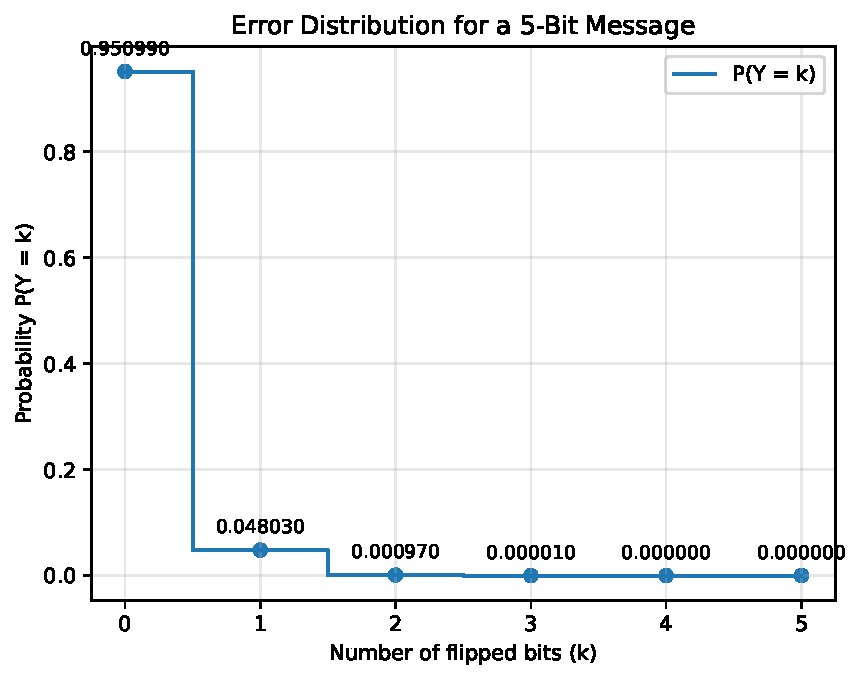
\includegraphics[width=0.75\linewidth]{figs/errordistri.pdf}
    \caption{Bit error probability distribution}
    \label{fig:cs1-2025-q20}
\end{figure}

\vspace{0.5cm}
% Question 21 (Q58)
\item Consider a probability distribution given by the density function $P(x)$:
\begin{align*}
P(x) = \begin{cases} C x^2, & \text{for } 1 \le x \le 4 \\ 0, & \text{for } x < 1 \text{ or } x > 4 \end{cases}
\end{align*}
The probability that $x$ lies between 2 and 3, i.e., $P(2 \le x \le 3)$ is \underline{\hspace{1cm}}.
\hfill (CS1~2025)

\vspace{0.2cm}
\solution
To find the probability using the Cumulative Distribution Function (CDF), we first determine the normalization constant $C$ by integrating the probability density function over its domain and setting the total integral equal to $1$:
\begin{align}
\int_1^4 C x^2 \, dx = 1 &\implies C \left[ \frac{x^3}{3} \right]_1^4 = 1 \\
                      &\implies C \left( \frac{64}{3} - \frac{1}{3} \right) = 1 \\
                      &\implies C = \frac{1}{21}
\end{align}

The Cumulative Distribution Function $F_X(x) = P(X \le x)$ represents the probability that the random variable $X$ takes a value less than or equal to $x$. It is obtained by integrating the PDF $P(t)$ from the lower bound $1$ up to $x$:
\begin{align}
F_X(x) = \int_1^x \frac{t^2}{21} \, dt = \left[ \frac{t^3}{63} \right]_1^x = \frac{x^3 - 1}{63} \quad \text{for } 1 \le x \le 4
\end{align}

Thus, the complete piecewise CDF is defined as:
\begin{align}
F_X(x) = \begin{cases} 
0, & x < 1 \\ 
\dfrac{x^3 - 1}{63}, & 1 \le x \le 4 \\ 
1, & x > 4 
\end{cases}
\end{align}

Using the fundamental property of the CDF, $P(a \le X \le b) = F_X(b) - F_X(a)$, the required probability that $x$ lies between 2 and 3 is evaluated as the difference between the CDF values at the upper and lower boundaries:
\begin{align}
P(2 \le X \le 3) &= F_X(3) - F_X(2) \\
                 &= \frac{3^3 - 1}{63} - \frac{2^3 - 1}{63} \\
                 &= \frac{26}{63} - \frac{7}{63} \\
                 &= \frac{19}{63} \approx 0.30158
\end{align}

The following Python code generates the CDF plot (\figref{fig:cs1-2025-q21-cdf}):
\begin{lstlisting}[frame=single, basicstyle=\rmfamily, escapeinside={(*@}{@*)}]
(*@\makebox[\dimexpr\linewidth-2\fboxsep-2\fboxrule\relax][c]{codes/cdf\_21.py}@*)
\end{lstlisting}
\begin{figure}[H]
    \centering
    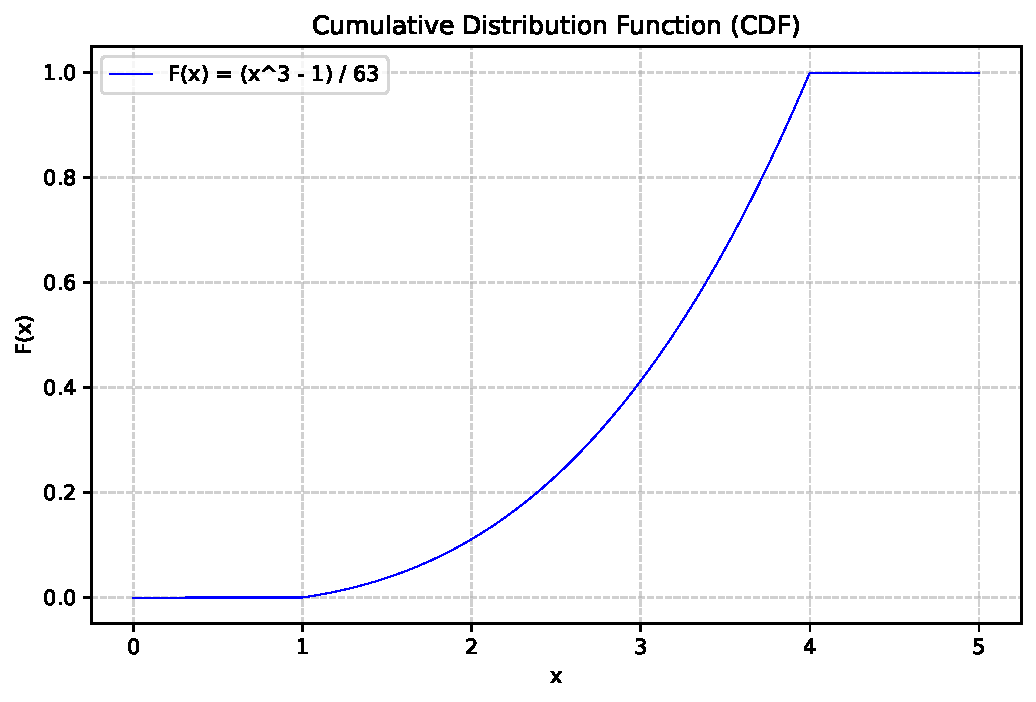
\includegraphics[width=0.75\linewidth]{figs/cdf_plot.pdf}
    \caption{Cumulative Distribution Function (CDF) plot}
    \label{fig:cs1-2025-q21-cdf}
\end{figure}

The following code gives the following figure (\figref{fig:cs1-2025-q21}).
\begin{lstlisting}[frame=single, basicstyle=\rmfamily, escapeinside={(*@}{@*)}]
(*@\makebox[\dimexpr\linewidth-2\fboxsep-2\fboxrule\relax][c]{codes/pdf\_21.py}@*)
\end{lstlisting}
\begin{figure}[H]
    \centering
    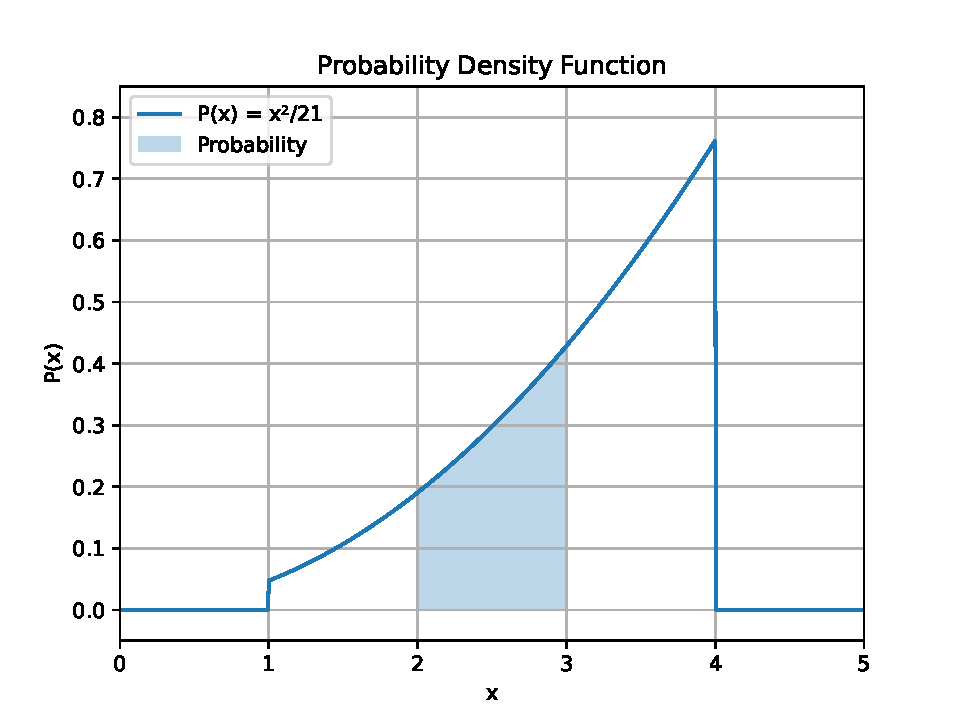
\includegraphics[width=0.75\linewidth]{figs/plt.pdf}
    \caption{Probability density function plot}
    \label{fig:cs1-2025-q21}
\end{figure}

The following code verifies the CDF plot by plotting random values and generates the following figure (\figref{fig:cdf-verify}).
\begin{lstlisting}[frame=single, basicstyle=\rmfamily, escapeinside={(*@}{@*)}]
(*@\makebox[\dimexpr\linewidth-2\fboxsep-2\fboxrule\relax][c]{codes/cdf\_verify.py}@*)
\end{lstlisting}
\begin{figure}[H]
    \centering
    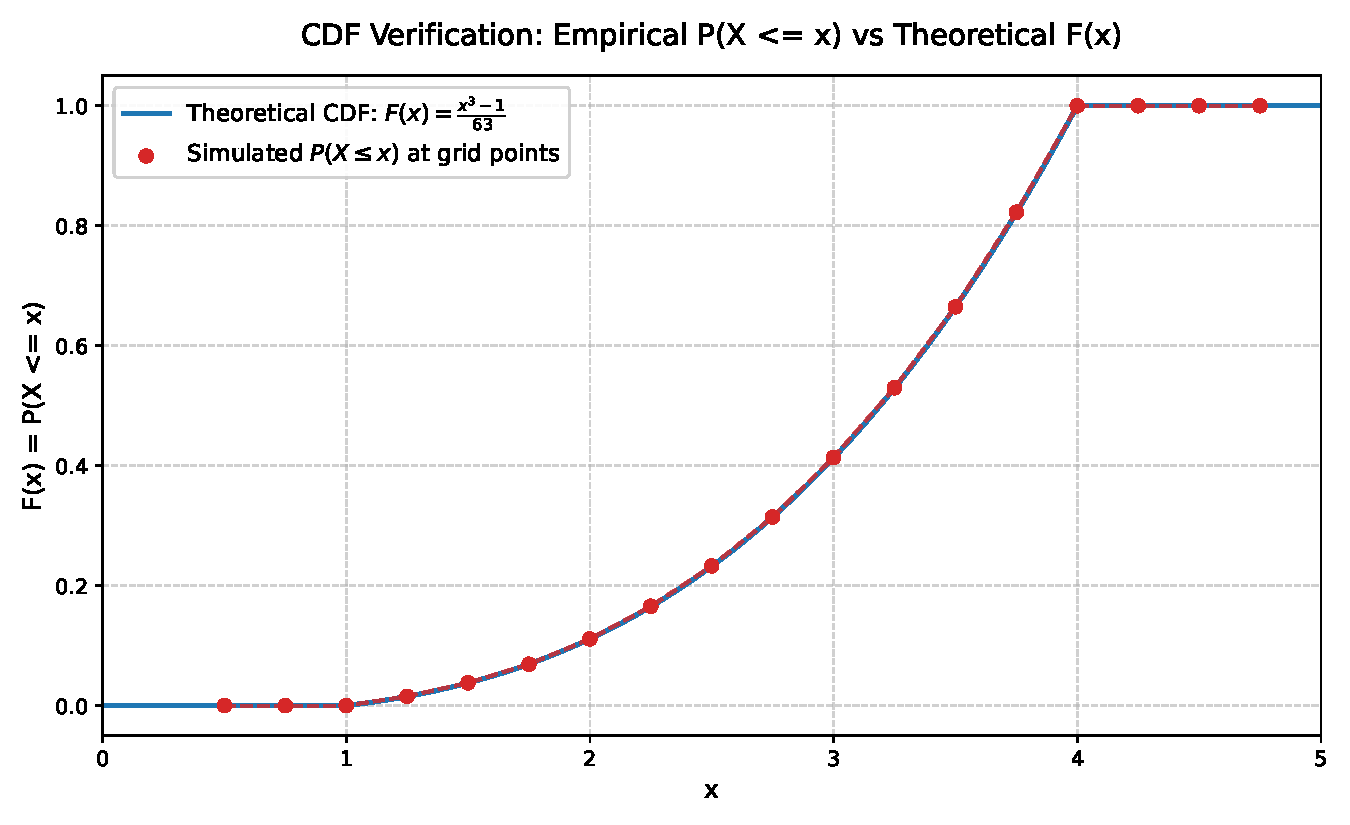
\includegraphics[width=0.75\linewidth]{figs/cdf_grid_verification.pdf}
    \caption{Cumulative Distribution Function (CDF) plot}
    \label{fig:cdf-verify}
\end{figure}

\vspace{0.5cm}
% Question 22 (Q59)
\item Consider the given finite state machine (FSM) with input $X$ and output $f$. The minimum number of states required to realize the FSM is to be determined.

\begin{center}
\renewcommand{\arraystretch}{1.1}
\begin{tabular}{|c|cc|cc|}
\hline
\multirow{2}{*}{Present state}
& \multicolumn{2}{c|}{Next state}
& \multicolumn{2}{c|}{Output $f$} \\
\cline{2-5}
& $X=0$ & $X=1$ & $X=0$ & $X=1$ \\
\hline
A & F & B & 0 & 0 \\
B & D & C & 0 & 0 \\
C & F & E & 0 & 0 \\
D & G & A & 1 & 0 \\
E & D & C & 0 & 0 \\
F & F & B & 1 & 1 \\
G & G & H & 0 & 1 \\
H & G & A & 1 & 0 \\
\hline
\end{tabular}

\end{center}

\solution

Grouping states with identical output pairs gives
\[
P_0=\{\{A,B,C,E\},\{D,H\},\{F\},\{G\}\}.
\]
Comparing their next-state groups splits $\{A,B,C,E\}$ into $\{A,C\}$ and $\{B,E\}$. The final partition is
\[
P=\{\{A,C\},\{B,E\},\{D,H\},\{F\},\{G\}\}.
\]
Hence, the minimized FSM has five states. Assign the codes
$S_0=000$, $S_1=001$, $S_2=010$, $S_3=011$ and $S_4=100$.

The minimized transition table, with separate rows for $X=0$ and $X=1$:

\begin{center}
\renewcommand{\arraystretch}{1.05}
\begin{tabular}{|c|c|c|c|c|}
\hline
Present state & $X$ & $Q_2Q_1Q_0$ & Next state code & $f$ \\
\hline
$S_0$ & 0 & 000 & 011 & 0 \\
$S_0$ & 1 & 000 & 001 & 0 \\
$S_1$ & 0 & 001 & 010 & 0 \\
$S_1$ & 1 & 001 & 000 & 0 \\
$S_2$ & 0 & 010 & 100 & 1 \\
$S_2$ & 1 & 010 & 000 & 0 \\
$S_3$ & 0 & 011 & 011 & 1 \\
$S_3$ & 1 & 011 & 001 & 1 \\
$S_4$ & 0 & 100 & 100 & 0 \\
$S_4$ & 1 & 100 & 010 & 1 \\
\hline
\end{tabular}

\end{center}

The state-transition diagram of the minimized FSM is shown in Fig.~\ref{fig:q22_fsm_diagram}. Each transition is labelled by its input $X$.

\begin{figure}[H]
    \centering
    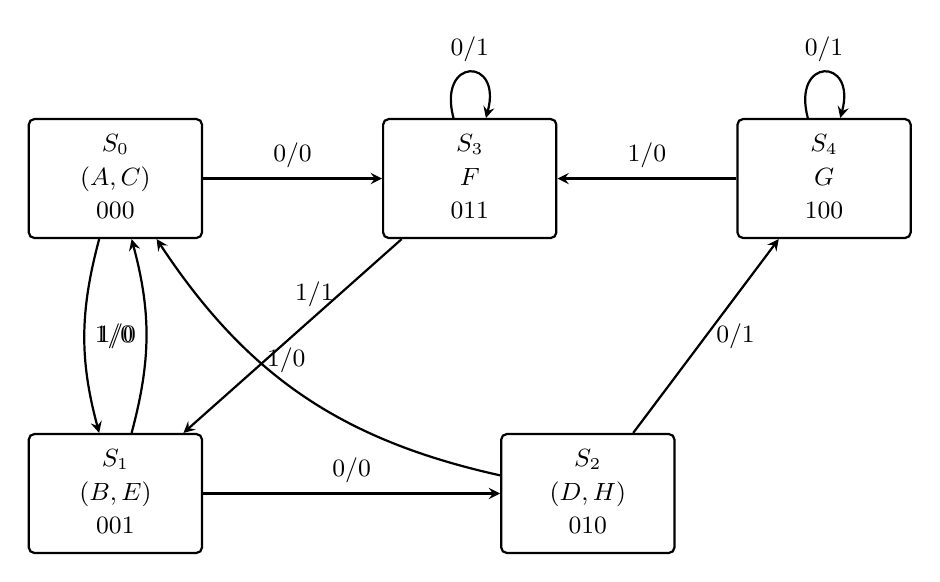
\begin{tikzpicture}[
    >=stealth,
    every node/.style={font=\small},
    state/.style={
        draw, rectangle, rounded corners=2pt, thick,
        align=center, minimum width=2.2cm,
        minimum height=1.1cm
    },
    every edge/.style={draw, thick, ->}
]
% Nodes positioning matching the handwritten layout using tabular for safe multi-line text
\node[state] (S0) at (0, 4) {\begin{tabular}{c} $S_0$ \\ $(A,C)$ \\ $000$ \end{tabular}};
\node[state] (S3) at (4.5, 4) {\begin{tabular}{c} $S_3$ \\ $F$ \\ $011$ \end{tabular}};
\node[state] (S4) at (9, 4) {\begin{tabular}{c} $S_4$ \\ $G$ \\ $100$ \end{tabular}};

\node[state] (S1) at (0, 0) {\begin{tabular}{c} $S_1$ \\ $(B,E)$ \\ $001$ \end{tabular}};
\node[state] (S2) at (6, 0) {\begin{tabular}{c} $S_2$ \\ $(D,H)$ \\ $010$ \end{tabular}};

% Transitions

% S0 <-> S1
\draw (S0) edge[bend right=15] node[right] {$1/0$} (S1);
\draw (S1) edge[bend right=15] node[left] {$1/0$} (S0);

% S0 -> S3
\draw (S0) edge node[above] {$0/0$} (S3);

% S1 -> S2
\draw (S1) edge node[above] {$0/0$} (S2);

% S2 -> S0 (Curved nicely to avoid overlapping with S3->S1 line)
\draw (S2) edge[bend left=22] node[above, pos=0.55] {$1/0$} (S0);

% S3 -> S1
\draw (S3) edge node[above, pos=0.4] {$1/1$} (S1);

% S2 -> S4
\draw (S2) edge node[right, pos=0.5] {$0/1$} (S4);

% S4 -> S3
\draw (S4) edge node[above] {$1/0$} (S3);

% Self-loop S3 (Above)
\draw (S3) edge[loop above, looseness=5] node[above] {$0/1$} (S3);

% Self-loop S4 (Above)
\draw (S4) edge[loop above, looseness=5] node[above] {$0/1$} (S4);

\end{tikzpicture}

    \caption{State-transition Diagram of Minimized FSM}
    \label{fig:q22_fsm_diagram}
\end{figure}

Therefore, the minimum number of states required is 5.

The following code verifies the solution:
\begin{lstlisting}[frame=single, basicstyle=\rmfamily, escapeinside={(*@}{@*)}]
(*@\makebox[\dimexpr\linewidth-2\fboxsep-2\fboxrule\relax][c]{codes/q22.c}@*)
\end{lstlisting}

\vspace{0.5cm}
% Question 23 (Q60)
\item Consider the given sequential circuit designed using D-Flip-flops. The circuit is initialized with some value (initial state). The number of distinct states the circuit will go through before returning back to the initial state is \underline{\hspace{1cm}}.
\hfill (CS1~2025)

\begin{figure}[H]
    \centering
    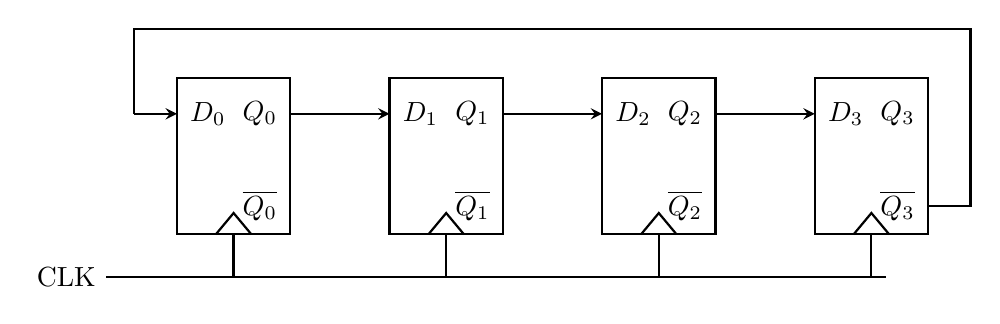
\begin{tikzpicture}[scale=0.9, >=stealth]
    \foreach \x/\i in {0/0, 3/1, 6/2, 9/3} {
        \draw[thick] (\x, 0) rectangle (\x+1.6, 2.2);
        \node[anchor=west] at (\x+0.05, 1.7) {$D_\i$};
        \node[anchor=east] at (\x+1.55, 1.7) {$Q_\i$};
        \node[anchor=east] at (\x+1.55, 0.4) {$\overline{Q_\i}$};
        \draw[thick] (\x+0.55, 0) -- (\x+0.8, 0.3) -- (\x+1.05, 0);
    }
    \draw[->, thick] (1.6, 1.7) -- (3.0, 1.7);
    \draw[->, thick] (4.6, 1.7) -- (6.0, 1.7);
    \draw[->, thick] (7.6, 1.7) -- (9.0, 1.7);
    \draw[thick] (10.6, 0.4) -- (11.2, 0.4) -- (11.2, 2.9) -- (-0.6, 2.9) -- (-0.6, 1.7);
    \draw[->, thick] (-0.6, 1.7) -- (0.0, 1.7);
    \draw[thick] (-1.0, -0.6) node[left] {CLK} -- (10.0, -0.6);
    \foreach \x in {0, 3, 6, 9} {
        \draw[thick] (\x+0.8, -0.6) -- (\x+0.8, 0.0);
    }
\end{tikzpicture}

\end{figure}

\vspace{0.2cm}
\solution
The given circuit is a 4-bit Johnson counter (twisted ring counter) constructed using four cascading D flip-flops, where the inverted output of the final stage is fed back to the first stage:
\begin{align}
D_0 = \overline{Q_3}, \quad D_1 = Q_0, \quad D_2 = Q_1, \quad D_3 = Q_2
\end{align}

Since $Q^+ = D$ for a D flip-flop, the next state function is:
\begin{align}
(Q_0, Q_1, Q_2, Q_3)^+ = (\overline{Q_3}, Q_0, Q_1, Q_2)
\end{align}

Starting from an initial state of $(0, 0, 0, 0)$, the circuit progresses through the following sequence of states:
\begin{align}
0000 \to 1000 \to 1100 \to 1110 \to 1111 \to 0111 \to 0011 \to 0001 \to 0000
\end{align}

Therefore, the circuit goes through 8 distinct states before returning to the initial state.

The following code verifies the solution:
\begin{lstlisting}[frame=single, basicstyle=\rmfamily, escapeinside={(*@}{@*)}]
(*@\makebox[\dimexpr\linewidth-2\fboxsep-2\fboxrule\relax][c]{codes/q23.c}@*)
\end{lstlisting}

\vspace{0.5cm}
% Question 24 (Q61)
\item Consider the following C program:
\begin{lstlisting}[language=C]
#include <stdio.h>

int foo (int S[], int size) {
    if (size == 0) return 0;
    if (size == 1) return 1;
    if (S[0] != S[1]) return 1 + foo(S + 1, size - 1);
    return foo(S + 1, size - 1);
}

int main() {
    int A[] = {0, 1, 2, 2, 2, 0, 0, 1, 1};
    printf ("%d", foo(A, 9));
    return 0;
}
\end{lstlisting}
The value printed by the given C program is \underline{\hspace{1cm}}.
\hfill (CS1~2025)

\vspace{0.2cm}
\solution
The function \texttt{foo(S, size)} recursively computes the total number of contiguous blocks (or runs) of identical elements in an array.

Mechanism of \texttt{foo(S, size)}:
\begin{itemize}
    \item If $S[0] \neq S[1]$, a boundary between two distinct contiguous blocks is detected, so it adds $1$ to the total count and recurses on $S+1$ with size $\text{size} - 1$.
    \item If $S[0] = S[1]$, the adjacent elements belong to the same contiguous block, so it recurses on $S+1$ without incrementing the count.
    \item The base case $\text{size} = 1$ returns $1$, accounting for the final contiguous block.
\end{itemize}

Tracing the execution step-by-step for $A = \{0, 1, 2, 2, 2, 0, 0, 1, 1\}$ with $\text{size} = 9$:
\begin{align}
\text{foo}(A, 9) &= 1 + \text{foo}(A+1, 8) && (A[0] \neq A[1], \text{ transition } 0 \to 1) \\
&= 1 + 1 + \text{foo}(A+2, 7) && (A[1] \neq A[2], \text{ transition } 1 \to 2) \\
&= 1 + 1 + \text{foo}(A+3, 6) && (A[2] = A[3] = 2) \\
&= 1 + 1 + \text{foo}(A+4, 5) && (A[3] = A[4] = 2) \\
&= 1 + 1 + 1 + \text{foo}(A+5, 4) && (A[4] \neq A[5], \text{ transition } 2 \to 0) \\
&= 1 + 1 + 1 + \text{foo}(A+6, 3) && (A[5] = A[6] = 0) \\
&= 1 + 1 + 1 + 1 + \text{foo}(A+7, 2) && (A[6] \neq A[7], \text{ transition } 0 \to 1) \\
&= 1 + 1 + 1 + 1 + \text{foo}(A+8, 1) && (A[7] = A[8] = 1)
\end{align}

At $\text{size} = 1$, the base case returns $\text{foo}(A+8, 1) = 1$:
\begin{align}
\text{foo}(A, 9) &= 1 + 1 + 1 + 1 + 1 \\
                 &= 5
\end{align}

Therefore, the value printed by the program is $5$.

\vspace{0.5cm}
% Question 25 (Q62)
\item Let \texttt{LIST} be a datatype for an implementation of linked list defined as follows:
\begin{lstlisting}[language=C]
typedef struct list {
    int data;
    struct list *next;
} LIST;
\end{lstlisting}
Suppose a program has created two linked lists, L1 and L2, whose contents are given in the figure below (code for creating L1 and L2 is not provided here). L1 contains 9 nodes, and L2 contains 7 nodes.

\begin{figure}[H]
    \centering
    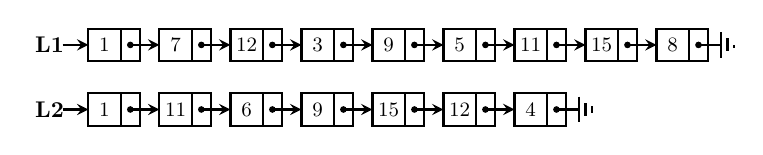
\begin{tikzpicture}[scale=0.82, transform shape, >=stealth]
    \node at (-0.6, 1) {\textbf{L1}};
    \draw[->, thick] (-0.4, 1) -- (0, 1);
    \foreach \val/\x in {1/0, 7/1.1, 12/2.2, 3/3.3, 9/4.4, 5/5.5, 11/6.6, 15/7.7, 8/8.8} {
        \draw[thick] (\x, 0.75) rectangle (\x+0.8, 1.25);
        \draw[thick] (\x+0.5, 0.75) -- (\x+0.5, 1.25);
        \node at (\x+0.25, 1) {\small \val};
        \filldraw (\x+0.65, 1) circle (1.2pt);
        \ifdim \x pt < 8.8pt
            \draw[->, thick] (\x+0.65, 1) -- (\x+1.1, 1);
        \fi
    }
    \draw[thick] (9.45, 1) -- (9.8, 1);
    \draw[thick] (9.8, 1.2) -- (9.8, 0.8);
    \draw[thick] (9.9, 1.1) -- (9.9, 0.9);
    \draw[thick] (10.0, 1.0) -- (10.0, 0.95);

    \node at (-0.6, 0) {\textbf{L2}};
    \draw[->, thick] (-0.4, 0) -- (0, 0);
    \foreach \val/\x in {1/0, 11/1.1, 6/2.2, 9/3.3, 15/4.4, 12/5.5, 4/6.6} {
        \draw[thick] (\x, -0.25) rectangle (\x+0.8, 0.25);
        \draw[thick] (\x+0.5, -0.25) -- (\x+0.5, 0.25);
        \node at (\x+0.25, 0) {\small \val};
        \filldraw (\x+0.65, 0) circle (1.2pt);
        \ifdim \x pt < 6.6pt
            \draw[->, thick] (\x+0.65, 0) -- (\x+1.1, 0);
        \fi
    }
    \draw[thick] (7.25, 0) -- (7.6, 0);
    \draw[thick] (7.6, 0.2) -- (7.6, -0.2);
    \draw[thick] (7.7, 0.1) -- (7.7, -0.1);
    \draw[thick] (7.8, 0.05) -- (7.8, -0.05);
\end{tikzpicture}

\end{figure}

\vspace{0.5cm}
Consider the following C program segment that modifies the list L1. The number of nodes that will be there in L1 after the execution of the code segment is \underline{\hspace{1cm}}.
\hfill (CS1~2025)
\begin{lstlisting}[language=C]
int find (int query, LIST *list) {
    while (list != NULL) {
        if (list->data == query) return 1;
        list = list->next;
    }
    return 0;
}

int main () {
    ptr1 = L1; ptr2 = L2;
    while (ptr1->next != NULL) {
        query = ptr1->next->data;
        if (find (query, L2))
            ptr1->next = ptr1->next->next;
        else
            ptr1 = ptr1->next;
    }
    return 0;
}
\end{lstlisting}

\vspace{0.2cm}
\solution
The code deletes every element in L1 (from $2^{\text{nd}}$ node onward) that appears in L2. Elements $12, 9, 11, 15$ are deleted from L1. Retained elements are $[1, 7, 3, 5, 8]$, leaving 5 nodes in total.

The following code can verify the solution:
\begin{lstlisting}[frame=single, basicstyle=\rmfamily, escapeinside={(*@}{@*)}]
(*@\makebox[\dimexpr\linewidth-2\fboxsep-2\fboxrule\relax][c]{codes/q25.c}@*)
\end{lstlisting}

\vspace{0.5cm}
% Question 26 (Q63)
\item Consider the following C program:
\begin{lstlisting}[language=C]
#include <stdio.h>

int gate (int n) {
    int d, t, newnum, turn;
    newnum = turn = 0; t = 1;
    while (n >= t) t *= 10;
    t /= 10;
    while (t > 0) {
        d = n / t;
        n = n % t;
        t /= 10;
        if (turn) newnum = 10 * newnum + d;
        turn = (turn + 1) % 2;
    }
    return newnum;
}

int main () {
    printf ("%d", gate (14362));
    return 0;
}
\end{lstlisting}
The value printed by the given C program is \underline{\hspace{1cm}}.
\hfill (CS1~2025)

\vspace{0.2cm}
\solution
The function \texttt{gate(n)} extracts the digits of $n$ from left to right and constructs a new integer \texttt{newnum} using alternate digits, starting from the second most significant digit (\texttt{turn = 1}).

For input $n = 14362$:
\begin{itemize}
    \item The first \texttt{while} loop calculates $t = 10000$, matching the place value of the most significant digit.
    \item The second \texttt{while} loop extracts digits from left to right and toggles \texttt{turn} at each step:
\end{itemize}

\begin{center}
\begin{tabular}{|c|c|c|c|c|}
\hline
Digit ($d$) & \texttt{turn} & Action & \texttt{newnum} & Next \texttt{turn} \\ \hline
1 & 0 & Skip & 0 & 1 \\
4 & 1 & Append $4$ & 4 & 0 \\
3 & 0 & Skip & 4 & 1 \\
6 & 1 & Append $6$ & 46 & 0 \\
2 & 0 & Skip & 46 & 1 \\ \hline
\end{tabular}

\end{center}

After iterating through all digits, the function returns \texttt{newnum} $= 46$.

Therefore, the value printed by the program is $46$.

\vspace{0.5cm}
% Question 27 (Q64)
\item The maximum value of $x$ such that the edge between the nodes B and C is included in every minimum spanning tree of the given graph is \underline{\hspace{1cm}}.
\hfill (CS1~2025)

\begin{figure}[H]
    \centering
    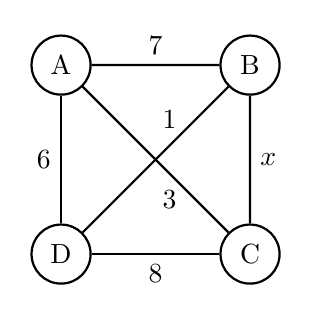
\begin{tikzpicture}[scale=1.2, >=stealth]
    \node[circle, draw, thick, minimum size=7.5mm, inner sep=0pt] (A) at (0, 2) {A};
    \node[circle, draw, thick, minimum size=7.5mm, inner sep=0pt] (B) at (2, 2) {B};
    \node[circle, draw, thick, minimum size=7.5mm, inner sep=0pt] (D) at (0, 0) {D};
    \node[circle, draw, thick, minimum size=7.5mm, inner sep=0pt] (C) at (2, 0) {C};

    \draw[thick] (A) -- node[above] {7} (B);
    \draw[thick] (A) -- node[left] {6} (D);
    \draw[thick] (D) -- node[below] {8} (C);
    \draw[thick] (B) -- node[right] {$x$} (C);

    \draw[thick] (D) -- node[pos=0.68, above left, fill=white, inner sep=1.5pt] {1} (B);
    \draw[thick] (A) -- node[pos=0.68, below left, fill=white, inner sep=1.5pt] {3} (C);
\end{tikzpicture}

\end{figure}

\vspace{0.2cm}
\solution
By the cut property of minimum spanning trees, an edge is included in every MST if it is the strictly unique minimum-weight edge crossing some cut. 

Consider the cut partitioning the vertices into $S = \{A, C\}$ and $V \setminus S = \{B, D\}$. The crossing edges and their weights are:
\begin{itemize}
    \item $(A, D) = 6$
    \item $(A, B) = 7$
    \item $(C, D) = 8$
    \item $(B, C) = x$
\end{itemize}

For edge $(B, C)$ to be the unique minimum-weight edge across this cut, its weight must be strictly less than the minimum of the other crossing edges:
\begin{align}
x < \min(6, 7, 8) \implies x < 6
\end{align}

Since $x$ must be an integer, the maximum value is $x = 5$.

\vspace{0.5cm}
% Question 28 (Q65)
\item In a double hashing scheme, $h_1(k) = k \bmod 11$ and $h_2(k) = 1 + (k \bmod 7)$ are the auxiliary hash functions. The size $m$ of the hash table is 11. The hash function for the $i$-th probe in the open address table is $[h_1(k) + i \cdot h_2(k)] \bmod m$. The following keys are inserted in the given order: 63, 50, 25, 79, 67, 24. The slot at which key 24 gets stored is \underline{\hspace{1cm}}.
\hfill (CS1~2025)

\vspace{0.2cm}
\solution
Using (\ref{eq:CS12025-double_hashing}), the auxiliary functions for key 24 are:
\begin{align}
h_1(24) &= 24 \bmod 11 = 2 \\
h_2(24) &= 1 + (24 \bmod 7) = 4
\end{align}
Keys 63, 50, 25, 79, 67 occupy slots 8, 6, 3, 2, 1 respectively.
\begin{itemize}
    \item $i=0$: $h(24, 0) = 2 \implies$ slot 2 occupied.
    \item $i=1$: $h(24, 1) = (2 + 4) \bmod 11 = 6 \implies$ slot 6 occupied.
    \item $i=2$: $h(24, 2) = (2 + 8) \bmod 11 = 10 \implies$ slot 10 empty.
\end{itemize}
Key 24 is stored at slot 10.

\end{enumerate}
